

\section{Method Overview}
\label{sec:method}

Given a rectified stereo pair $\mathbf{I}_L, \mathbf{I}_R \in \mathbb{R}^{3 \times H \times W}$, we first obtain monocular depth estimates (MDEs) $\mathbf{M}_L, \mathbf{M}_R \in \mathbb{R}^{1 \times H \times W}$ using a generic VFM $\phi_M$ for monocular depth estimation. We aim to estimate a disparity map $\mathbf{D}=\phi_S(\mathbf{I}_L, \mathbf{I}_R, \mathbf{M}_L, \mathbf{M}_R)$, incorporating VFM priors to provide accurate results even under challenging conditions, such as texture-less areas, occlusions, and non-Lambertian surfaces. 
At the same time, our stereo network $\phi_S$ is designed to avoid depth estimation errors that could arise from relying solely on contextual cues, which can be ambiguous, like in the presence of visual illusions.

Following recent advances in iterative models \cite{lipson2021raft}, \method comprises three main stages, as shown in \cref{fig:arch}: I) Feature Extraction, II) Correlation Pyramids Building, and III) Iterative Disparity Estimation.

\subsection{Feature Extraction}

Two distinct types of features are extracted \cite{lipson2021raft}: image features and context features -- (1) and (6) in \cref{fig:arch}.
The image features are obtained through a feature encoder processing the stereo pair, yielding feature maps $\mathbf{F}_L, \mathbf{F}_R \in \mathbb{R}^{D \times \frac{H}{4} \times \frac{W}{4}}$, which are used to build a stereo correlation volume at $\frac{1}{4}$ of the original input resolution.
These encoders are initialized with pre-trained weights \cite{lipson2021raft} and the image encoder is kept frozen during training.
For context features, we employ a context encoder with identical architecture to the feature encoder, but processing the monocular depth estimate aligned with the reference image $\mathbf{M}_L$ -- (3) in \cref{fig:arch} -- instead of $\mathbf{I}_L$ to capture strong geometry priors. Accordingly, during training the context encoder is optimized to extract meaningful features from these depth maps.

\subsection{Correlation Pyramids Building}
\label{subsec:corr_pyramids}

As a standard practice in stereo matching, the \textit{cost volume} is the data structure encoding the similarity between pixels across the two images. Accordingly, our model makes use of cost volumes -- in particular, of Correlation Pyramids \cite{lipson2021raft} -- yet in a different manner.
Indeed, \method builds two correlation pyramids, respectively a \textit{stereo correlation volume} starting from $\mathbf{I}_L, \mathbf{I}_R$ to encode image similarities, and a \textit{monocular correlation volume} from $\mathbf{M}_L, \mathbf{M}_R$ to encode geometric similarities -- (2) and (4) in \cref{fig:arch}. 
Conversely to the former, the latter will not be influenced by non-Lambertian surfaces, assuming a strong $\phi_M$.

\textbf{Stereo Correlation Volume.} Given $\mathbf{F}_L, \mathbf{F}_R$, we construct a 3D correlation volume $\mathbf{V}_S$ using dot product between feature maps:
\begin{equation}
    (\mathbf{V}_S)_{ijk} = \sum_{h} (\mathbf{F}_L)_{hij} \cdot (\mathbf{F}_R)_{hik}, \ \mathbf{V}_S \in \mathbb{R}^{\frac{H}{4} \times \frac{W}{4} \times \frac{W}{4}}
    \label{eq:dot_corr}
\end{equation}

\textbf{Mononocular Correlation Volume.} Given $\mathbf{M}_L, \mathbf{M}_R$, 
we downsample them to 1/4, compute their normals $\nabla_L, \nabla_R$,
and construct a 3D correlation volume $\mathbf{V}_M$ using dot product between normal maps:
\begin{equation}
    (\mathbf{V}_M)_{ijk} = \sum_{h} (\nabla_L)_{hij} \cdot (\nabla_R)_{hik}, \ \mathbf{V}_M \in \mathbb{R}^{\frac{H}{4} \times \frac{W}{4} \times \frac{W}{4}}
    \label{eq:dot_corr_mono}
\end{equation}

Given the absence of texture in $\nabla_L$ and $\nabla_R$, the resulting monocular volume $\mathbf{V}_M$ will be less informative. 
To alleviate this problem we segment $\mathbf{V}_M$ using the relative depth priors from $\mathbf{M}_L$ and $\mathbf{M}_R$: to do so, we generate left and right segmentation masks $\mathcal{M}_L \in \{0,1\}^{\frac{H}{4} \times \frac{W}{4} \times 1}$, $\mathcal{M}_R \in \{0,1\}^{\frac{H}{4} \times 1 \times \frac{W}{4}}$.
We refer the reader to the \textbf{supplementary material} for a detailed description.
Given the segmentation masks, we can generate masked volumes as:
\begin{equation}
    ({\mathbf{V}_M}^n)_{ijk} = ({\mathcal{M}_L}^n)_{ij} \cdot ({\mathcal{M}_R}^n)_{ik} \cdot (\mathbf{V}_M)_{ijk}
    \label{eq:vol_masking}
\end{equation}
Next, we insert a 3D Convolutional Regularization module $\phi_A$ to aggregate ${\mathbf{V}_M}^n$, resulting in ${\mathbf{V}'}_M=\phi_A({\mathbf{V}_M}^1,\dots,{\mathbf{V}_M}^{N},\mathbf{M}_L,\mathbf{M}_R)$, with $N=8$. The architecture of $\phi_A$ follows the one in \cite{xu2023iterative}, with a simple permutation to match the structure of the correlation volumes.
We propose an adapted version of CoEx \cite{bangunharcana2021correlate} correlation volume excitation that exploits both views. 
The resulting feature volumes ${\mathbf{V}'}_M \in \mathbb{R}^{F \times \frac{H}{4} \times \frac{W}{4} \times \frac{W}{4}}$ are fed to two different shallow 3D conv layers $\phi_D$ and $\phi_C$ to obtain two aggregated volumes $\mathbf{V}^D_M = \phi_D({\mathbf{V}'}_M)$ and $\mathbf{V}^C_M = \phi_C({\mathbf{V}'}_M)$ with $\mathbf{V}^D_M,\mathbf{V}^C_M \in \mathbb{R}^{\frac{H}{4} \times \frac{W}{4} \times \frac{W}{4}}$.

\textbf{Differentiable Monocular Scaling.} Volume $\mathbf{V}^D_M$ will be used not only as a monocular guide for the iterative refinement unit but also to estimate the coarse disparity maps $\hat{\mathbf{D}}_L$ $\hat{\mathbf{D}}_R$, while $\mathbf{V}^C_M$ is used to estimate confidence maps $\hat{\mathbf{C}}_L$ $\hat{\mathbf{C}}_R$: those maps are used to scale both $\mathbf{M}_L$ and $\mathbf{M}_R$ -- (5) in \cref{fig:arch}. 
To estimate left disparity from a correlation volume, we can first perform a \textit{softargmax} on the last $W$ dimension of $\mathbf{V}^D_M$ to extract the correlated pixel x-coordinate, then given the relationship between left disparity and correlation $d_L=j_L-j_R$ we obtain a coarse disparity map $\hat{\mathbf{D}}_L$: 
\begin{equation} 
    (\hat{\mathbf{D}}_L)_{ij} = j - \text{softargmax}_L(\mathbf{V}^D_M)_{ij}
    \label{eq:softmax_left}
\end{equation}
Similarly, we can estimate $\hat{\mathbf{D}}_R$ from $\mathbf{V}^D_M$. We refer the reader to the supplementary for details.
We also aim to estimate a pair of confidence maps $\hat{\mathbf{C}}_L, \hat{\mathbf{C}}_R \in [0,1]^{H \times W}$ to classify outliers and perform a robust scaling.
Inspired by information entropy, we estimate the \textit{chaos} inside correlation curves: clear monomodal-like cost curve -- \ie, the ones with low entropy -- are reliable -- while \textit{chaotic} curves -- \ie, the ones with high entropy -- are uncertain.
To estimate the left confidence map, we perform a \textit{softmax} operation on the last $W$ dimension of $\mathbf{V}^C_M$, then $\hat{\mathbf{C}}_L$ is obtained as follows:
\begin{equation}
    (\hat{\mathbf{C}}_L)_{ij} = 1  + \frac{\sum_{d}^{\frac{W}{4}} \frac{e^{(\mathbf{V}^C_M)_{ijd}}}{\sum_{f}^{\frac{W}{4}} e^{(\mathbf{V}^C_M)_{ijf}}} \cdot \log_2 \left( \frac{e^{(\mathbf{V}^C_M)_{ijd}}}{\sum_{f}^{\frac{W}{4}} e^{(\mathbf{V}^C_M)_{ijf}}} \right)}{\log_2(\frac{W}{4})}
    \label{eq:confidence_left}
\end{equation}
In the same way, we estimate $\hat{\mathbf{C}}_R$.
To further reduce outliers, we mask out from $\hat{\mathbf{C}}_L$ and $\hat{\mathbf{C}}_R$ occluded pixels using a \textit{SoftLRC} operator -- see the \textbf{supplementary material} for details.
Finally, we can estimate the scale $\hat{s}$ and shift $\hat{t}$ using a differentiable weighted least-square approach:
\begin{equation}
    \min_{\hat{s}, \hat{t}} \sum_{}^{L,R} \left\lVert \sqrt{\hat{\mathbf{C}}}\odot\left[\left(\hat{s}\mathbf{M} + \hat{t}\right)  - \hat{\mathbf{D}} \right] \right\rVert_F 
    \label{eq:scale_shift}
\end{equation}
where $\lVert\cdot\rVert_F$ denotes the Frobenius norm.
Using the scaling coefficients, we obtain two disparity maps $\hat{\mathbf{M}}_L$, $\hat{\mathbf{M}}_R$:
\begin{equation}
    \hat{\mathbf{M}}_L = \hat{s}\mathbf{M}_L + \hat{t},\ \hat{\mathbf{M}}_R = \hat{s}\mathbf{M}_R + \hat{t}
    \label{eq:scaling_op}
\end{equation}
It is crucial to optimize both left and right scaling jointly to obtain consistency between $\hat{\mathbf{M}}_L$ and $\hat{\mathbf{M}}_R$.

\begin{figure*}[t]
    \centering
    \renewcommand{\tabcolsep}{1pt}
    \hspace*{-0.5cm}\begin{tabular}{ccccccc}
    \small Image
    & \small Ground-Truth
    & \small Depth Anything v2 \cite{depth_anything_v2} & 
    & \small Image
    & \small Ground-Truth
    & \small Depth Anything v2 \cite{depth_anything_v2} \\
    
    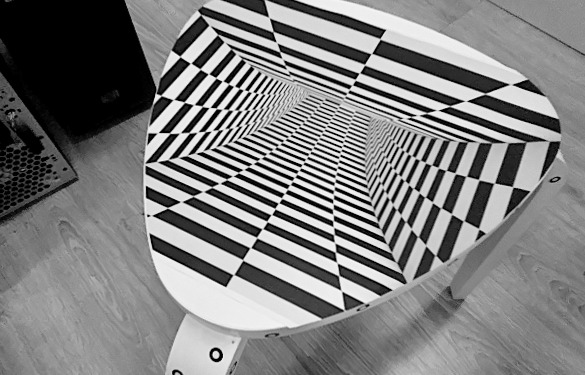
\includegraphics[width=0.16\textwidth]{imgs/monotrap_samples/rgb/13.jpg}
    &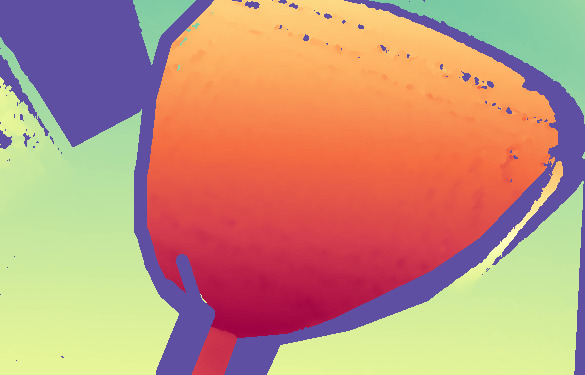
\includegraphics[width=0.16\textwidth]{imgs/monotrap_samples/gt/13.jpg}
    &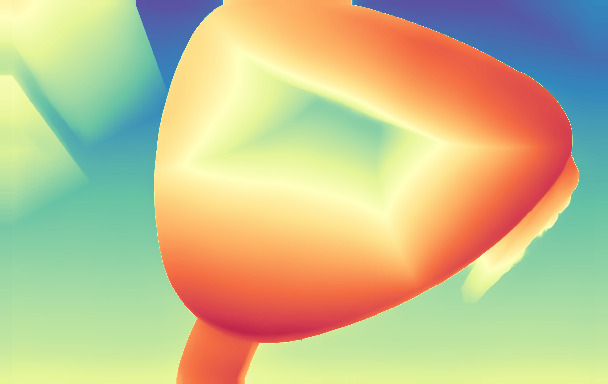
\includegraphics[width=0.16\textwidth]{imgs/monotrap_samples/mono/13.jpg}
    & \hspace{0.1cm} &

    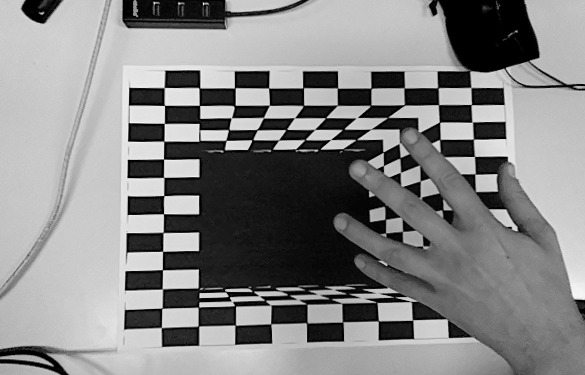
\includegraphics[width=0.16\textwidth]{imgs/monotrap_samples/rgb/2.jpg}
    &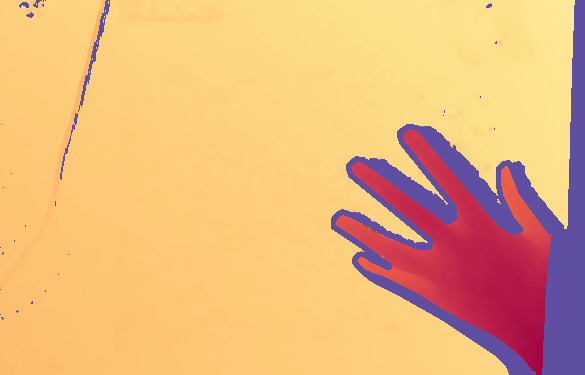
\includegraphics[width=0.16\textwidth]{imgs/monotrap_samples/gt/2.jpg}
    &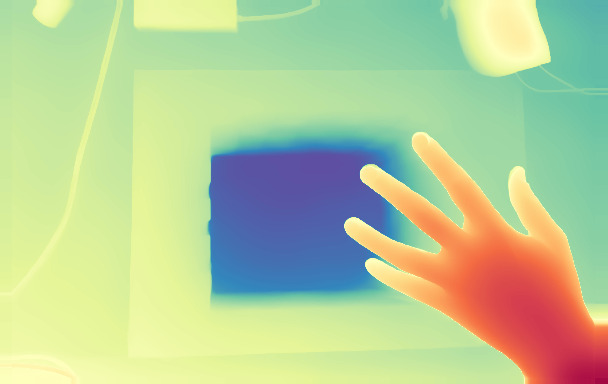
\includegraphics[width=0.16\textwidth]{imgs/monotrap_samples/mono/2.jpg}
    \\
    \end{tabular}\vspace{-0.2cm}
    \caption{\textbf{Samples from \dataset Dataset.} We report two scenes featured in our dataset, showing the left image, the ground-truth depth, and the predictions by Depth Anything v2 \cite{depth_anything_v2}, highlighting how it fails in the presence of visual illusions.}\vspace{-0.3cm}
    \label{fig:monotrap}
\end{figure*}

\textbf{Volume Augmentations.} Unfortunately, \method cannot properly learn when to choose stereo or mono information from \cite{mayer2016large} alone.
Hence, we propose three volume augmentations and a monocular augmentation to overcome this issue: 1) \textit{Volume Rolling}: we randomly apply a rolling operation to the last $W$ dimension of ${\mathbf{V}^D}_M$ or ${\mathbf{V}}_S$; 2) \textit{Volume Noising}: we apply random noise sampled from the interval $[0,1)$ using a uniform distribution; 3) \textit{Volume Zeroing}: we apply a Gaussian-like curve with the peak where disparity equals zero. Furthermore, we randomly substitute the monocular prediction with the ground truth normalized between $[0,1]$ as an additional augmentation.
We apply only one volume augmentation to ${\mathbf{V}^D}_M$ or ${\mathbf{V}}_S$ and only for a section of the volume, randomly selecting an $\mathcal{M}_L^n$ mask.

\textbf{Volume Truncation.} To further help \method to handle mirror surfaces, we introduce a hand-crafted volume truncation operation on ${\mathbf{V}}_S$. Firstly, we extract left confidence $\mathbf{C}_M=\text{softLRC}_L(\hat{\mathbf{M}}_L, \hat{\mathbf{M}}_R)$ to classify reliable monocular predictions. Then, we create a truncate mask $\mathbf{T} \in [0,1]^{\frac{H}{4} \times \frac{W}{4}}$ using the following logic condition: $(\mathbf{T})_{ij}=\left[\left((\hat{\mathbf{M}}_L)_{ij} >(\hat{\mathbf{D}}_L)_{ij}\right) \land (\mathbf{C}_M)_{ij} \right] \lor \left[ (\mathbf{C}_M)_{ij} \land \neg(\hat{\mathbf{C}}_L)_{ij} \right]$.
We implement this logic using fuzzy operators (more details in the \textbf{supplementary material}).
The rationale is that stereo predicts farther depths on mirror surfaces: the mirror is perceived as a window on a new environment, specular to the real one.
Finally, for values of $\mathbf{T}>T_\text{m}=0.98$, we truncate ${\mathbf{V}_S}$ using a sigmoid curve centered at the correlation value predicted by $\hat{\mathbf{M}}_L$ -- \ie, the real disparity of mirror surfaces -- preserving only the stereo correlation curve that does not ``pierce" the mirror region.

\subsection{Iterative Disparity Estimation}

We aim to estimate a series of refined disparity maps $\{\mathbf{D}^1=\hat{\mathbf{M}}_L, \mathbf{D}^2,\dots\,\mathbf{D}^l,\dots\}$ exploiting the guidance from both stereo and mono branches. 
Starting from the Multi-GRU update operator by \cite{lipson2021raft}, we introduce a second lookup operator that extracts correlation features $\mathbf{G}_M$ from the additional volume $\mathbf{V}^D_M$ -- (7) in \cref{fig:arch}.
The two sets of correlation features from $\mathbf{G}_S$ and $\mathbf{G}_M$ are processed by the same two-layer encoder and concatenated with features derived from the current disparity estimation $\mathbf{D}^l$. This concatenation is further processed by a 2D conv layer, and then by the ConvGRU operator.
We inherit the convex upsampling module \cite{lipson2021raft} to upsample final disparity to full resolution.

\subsection{Training Supervision}
We supervise the iterative module using the well-known L1 loss with exponentially increasing weights \cite{lipson2021raft}, then $\hat{\mathbf{D}}_L$, $\hat{\mathbf{D}}_R$, $\hat{\mathbf{M}}_L$ and $\hat{\mathbf{M}}_R$ using the L1 loss, 
finally $\hat{\mathbf{C}}_L$ and $\hat{\mathbf{C}}_R$ using the Binary Cross Entropy loss.
We invite the reader to read the \textbf{supplementary material} for additional details.

\begin{table*}[t]
\centering
\renewcommand{\tabcolsep}{12pt}
\scalebox{0.72}{
\begin{tabular}{|ll|rrrrr|rrrr|}
\multicolumn{2}{c}{} & \multicolumn{5}{c}{Booster (Q)} & \multicolumn{4}{c}{Middlebury 2014 (H)} \\ 
\hline
 & \multirow{2}{*}{Experiment} & \multicolumn{4}{c}{bad} & Avg. & \multicolumn{3}{c}{bad $>2$} & Avg. \\
 & & $>2$ & $>4$ & $>6$ & $>8$ & (px) & All & Noc & Occ & (px) \\
\hline\hline

(A) & Baseline \cite{lipson2021raft}
& 17.86 & 13.09 & 10.76 & 9.24 & 3.58
& 11.15 & 8.06 & 29.06 & 1.55 \\
\hline\hline
(B) & (A) + Monocular Context w/o re-train
& 15.85 & 10.98 & 8.89 & 7.69 & 3.05
& 14.96 & 11.70 & 34.38 & 2.82 \\
(C) & (A) + Monocular Context w/ re-train
& \trd 14.94 & \trd 10.40 & \trd 8.61 & \trd 7.63 & \trd 3.03
& \trd 9.62 & \trd 6.98 & \trd 25.39 & \trd 1.13 \\
(D) & (C) + Normals Correlation Volume / Scaled Depth
& \snd 11.33 & \snd 6.88 & \snd 5.32 & \snd 4.59 & \snd 1.87
& \snd 7.67 & \snd 5.24 & \snd 21.51 & \fst 0.96 \\
(E) & (D) + Volume augmentation / truncation
& \fst 9.96 & \fst 5.81 & \fst 4.48 & \fst 3.79 & \fst 1.36
& \fst 7.07 & \fst 4.76 & \fst 20.77 & \snd 0.97 \\
\hline
\end{tabular}}\vspace{-0.2cm}
\caption{\textbf{Ablation Studies.} We measure the impact of different design strategies. Networks trained on SceneFlow \cite{mayer2016large}.
}
\label{tab:ablation}
\end{table*}

\section{The \dataset Dataset}

Monocular depth estimation is known for possibly failing in the presence of perspective illusions.
The reader may wonder how \method would behave in such cases: would it blindly trust the monocular VFM or rely on the stereo geometric principles to maintain robustness?

To answer these questions, we introduce MonoTrap, a novel stereo dataset specifically designed to challenge monocular depth estimation. Our dataset comprises 26 scenes featuring perspective illusions, captured with a calibrated stereo setup and annotated with ground-truth depth from an Intel Realsense L515 LiDAR.
The scenes contain carefully designed planar patterns that create visual illusions, such as apparent holes in walls or floors and simulated transparent surfaces that reveal content behind them. 
Figure \ref{fig:monotrap} shows examples from our dataset that illustrate how these visual illusions easily fool monocular methods. 
